\documentclass[10pt]{article}

\usepackage[english]{babel}										
                                                               
\usepackage[utf8]{inputenc}										
\usepackage[T1]{fontenc}										

\usepackage{amsmath,amsfonts,amssymb,amsthm,cancel,siunitx,
calculator,calc,mathtools,empheq,latexsym}

\usepackage{subfig,epsfig,tikz,float}

\usepackage{booktabs,multicol,multirow,tabularx,array}

\usepackage{hyperref}
\usepackage{natbib}

\usepackage{xcolor}
\usepackage{listings}

\definecolor{mGreen}{rgb}{0,0.6,0}
\definecolor{mGray}{rgb}{0.5,0.5,0.5}
\definecolor{mPurple}{rgb}{0.58,0,0.82}
\definecolor{backgroundColour}{rgb}{0.95,0.95,0.92}

\lstdefinestyle{CStyle}{
    backgroundcolor=\color{backgroundColour},   
    commentstyle=\color{mGreen},
    keywordstyle=\color{magenta},
    numberstyle=\tiny\color{mGray},
    stringstyle=\color{mPurple},
    basicstyle=\footnotesize,
    breakatwhitespace=false,         
    breaklines=true,                 
    captionpos=b,                    
    keepspaces=true,                 
    numbers=left,                    
    numbersep=5pt,                  
    showspaces=false,                
    showstringspaces=false,
    showtabs=false,                  
    tabsize=2,
    language=C
}

\sloppy
\setlength{\parindent}{0pt}
\setlength{\parskip}{5pt}
\textwidth 13.5cm
\textheight 19.5cm
\columnsep .5cm

\title{\renewcommand{\baselinestretch}{1.17}\normalsize\bf%
\uppercase{PageRank, HITS and INDEGREE}
}

\author{
Giacomo Zanatta - 859156
}

\begin{document}

\date{}

\maketitle

\vspace{-0.5cm}

\begin{center}
{\footnotesize 
IRWS Project - Ca' Foscari University, Venice 
}
\end{center}

% -------------------------------------------------------------------
% Abstract
\bigskip
\noindent
{\small
\url{https://github.com/giacomozanatta/pagerank-hits}
}
\iffalse
\medskip
\noindent
{\small{\bf Keywords}{:} 
}
\fi

\baselineskip=\normalbaselineskip
% -------------------------------------------------------------------

\section{Introduction}\label{sec:1}
The project \cite{Zanatta_Page_Rank_HITS_2022} will show the computation of {\bf PageRank}\cite{Page98thepagerank} and {\bf HITS}\cite{Kleinberg1999} ranking algorithm and how these rankings are similiar.

The implementation was written in {\bf C language} with extensibility in mind: effort was made in order to write a library prototype that can be easily expanded adding for example other distance functions or different ranking algorithms.

Since we are dealing with large datasets, the underlying adjancency matrices are represented in a {\bf Compressed Row Storage} (from now, CSR) form in addition to the {\bf mmap} support.

This report is subdivided in 3 main chapter.  
In this section we will provide a brief introduction about the implemented algorithms, giving an high level overview.\\
In the next chapter we discuss about the implementation dissecting the library file and we show an example of utilization.\\
On the last chapter we present some results, comparing the generated ranking using the Jaccard similarity.

\subsection{Algorithms}
Here we will explain the main algorithms used for the project.
\subsubsection{PageRank}
PageRank is an algorithm used by Google Search Engine to measure the quality and importance of a page. It assigns a weight on every pages of a graph.
The PageRank algorithm outputs a probability distribution used to represent the likelihood that a person randomly clicking on links will arrive at any particular page.
Weights are expressed in percentage, for example a weight of 0.1 on page A means that a surfer has 10\% probability of reaching the page A by clicking a random link.
An hyperlink from page A to B can be seen as a vote by page A to page B. Vote casted by important pages weight more heavily and help to make other pages more important.
A page has a prestige level based on how many inlinks it has.
The PageRank score of page i is defined by:

$P(i)=\sum_{(j,i) \in E}\frac{P(j)}{O_j}$

where $P(j)$ is the PageRank score of page j and $O_j$ is the number of out links of j.

Page Rank can be computed using the Power iteration method: we start assigning at each page a score $P_{0}$ of 1/(number of nodes). We define A, the transition matrix of the graph, as:

$A_{ij} = \begin{cases} \frac{1}{0_j} & \mbox{if } (i,j) \in E \\ 0 & \mbox{otherwise}\end{cases}$

Since many pages have no out-links (some rows have all zeros), we can remove it from the computation.  
Note that the matrix is aperiodic. We can fix this by adding a dumping factor d: with probability d, a random surfer randomly chooses an out-link to follow. With probability 1-d instead, it will jump to a random page (teleportation).
An improved PageRank equation that take this into account is:

$P=((1-d)E/n+dA^T)P$

Where E is a n*n square matrix with every entry setted to 1/n (n is the number of nodes).
Using power iteration, the PageRank vector at iteration k+1 is computed as:

$P_{k+1} = (1-d)e/n+dA^TP_k$

Where $P_0$ is a vector of all 1's.
The value of d is 0.85. This is used in the PageRank paper.
\subsubsection{HITS}
HITS (Hypertext Induced Topic Search) is a query-dependent ranking and it is based on the idea of Authority and Hub pages: an authority is a page with many inlinks. An hub is a page with many outlinks.
Hubs and Authority has a mutual reinforcement relationships: an hub is good if it has a lot of outgoing links to good authority. On the other hand, a good authority wants in-links from good hubs.
HITS assigns two score at every page: authority score and hub score.

The adjacency matrix of the graph is defined by the matrix L:

$L_{ij} = \begin{cases} 1 & \mbox{if } (i,j) \in E \\ 0 & \mbox{otherwise}\end{cases}$

The authority of a page i, a(i), is: $a(i)=\sum_{(j,i) \in E}h(j)$. 

The hub of a page i, h(i), is: $h(i)=\sum_{(i,j) \in E}a(j)$.

In matrix notation, we can write:

$a = L^Th$

$h = La$

where a, h are the column vectors that contains, respectively, the authority and hub scores of each page.
Using the Power iteration method and starting with $a_0=h_0=(1,1,1,1,....,1)$, the final solutions are:

$a_k = L^TLa_{k-1}$

$h_k = LL^Th_{k-1}$

\subsubsection{In-Degree}
The indegree ranking simply counts how many ingoing link a page has. For computing indegree score for a page, we can take the transpose of the adjacency matrix and count for a page X how many indegree it has, then we divide the sum by the number of total nodes.
\subsubsection{Jaccard Similarity}
Jaccard similarity between two ranks A and B can be computed by this formula:

$J(A,B) = \frac{|A \cap B|}{|A \cup B|}$

That is in other words the number of different elements in A and B (intersection) divided by the total number of elements in the two set. Since the two sets have the same size, this is calculated as 2*(size of set).
\section{Implementation}
\subsection{Input data}
A ranking algorithms works with a set of pages. Every page could have a set of outgoing links. An outgoing links represents a link from a page to another one. 

We can model this by using a directed graph: a page is a node of the graph and an directed edge from page x to page y means that page x has an outgoing link to page y.

Network graph is taken from a text file, we assume that a file is structured as a follows:

\begin{enumerate}
    \item {\bf Must starts with an Header}. Header lines begins with the {\bf \texttt{\#}} character. Header contains useful information like the number of nodes and the number of edges of the graph stored in a special line structured like this:
    \begin{verbatim} # Nodes: X Edges: Y \end{verbatim}
    Where X and Y are two integers that represents respectively the number of nodes and the number of edges.
    File must have only one Header section.
    \item {\bf Must contains a number of edges that matches the number specified in the header}. After the section header, file must contains Y lines (where Y is the number of edges). An edge of the graph is defined by a line in the file. A line after the header must be in the next format:
    \begin{verbatim}A B\end{verbatim}
    Where A and B are two integers. A line in the file says that page identified by ID A has an outgoing link to the page identified by id B. 
    For better understandability, we call A FROMNODEID and B TONODEID
    \item {\bf Edges entry must be ordered}. The entry of the file must be sorted first by the first integer of the line and then by the second one.
\end{enumerate}
Here we provide a simple example of a valid file.
\begin{verbatim}
# Test graph
# Nodes: 8 Edges: 14
# FromNodeId	ToNodeId
0 3
1 2
1 4
2 0
3 1
4 1
4 2
4 3
4 5
5 2
5 7
6 0
6 2
7 0
\end{verbatim}
\subsection{Matrix representation}
The previous example corresponds to the next adajcency matrix:

$ \begin{bmatrix}
    0 & 0 & 0 & 1 & 0 & 0 & 0 & 0 \\
    0 & 0 & 1 & 0 & 1 & 0 & 0 & 0 \\
    1 & 0 & 0 & 0 & 0 & 0 & 0 & 0 \\
    0 & 1 & 0 & 0 & 0 & 0 & 0 & 0 \\
    0 & 1 & 1 & 1 & 0 & 1 & 0 & 0 \\
    0 & 0 & 1 & 0 & 0 & 0 & 0 & 1 \\
    1 & 0 & 1 & 0 & 0 & 0 & 0 & 0 \\
    1 & 0 & 0 & 0 & 0 & 0 & 0 & 0 
    \end{bmatrix}  $

Storing this matrix in a standard matrix representation requires $8*8 = 64$ entries.

Problem arises when we have to work with huge dataset: some network has {\bf millions of nodes} and this requires a lot of space.

For example, if we store entries as a float (4 bytes) a network with 50.000 nodes has 2.500.000.000 entries and we need 4*2.500.000.000 bytes (10 gigabytes) for store them.

Since large matrix are very sparse (we assume that a page contains only a few outgoing links) we can store the matrix in a CSR format.
\subsubsection{CSR format}
Matrices in CSR format are expressed by three one-dimensional array \cite{DongarraSparseMatrix}: one array (val) contains the non-zero values of the matrix. Another array (col\_index) is used to store the column indexes of the elements in the val vector. The last vector (row\_ptr) stores the locations in the val vector that start a row. In a more specific say:
\begin{enumerate}
    \item The arrays val and col\_index are of length N (number of total non-zero values in matrix), and contain the non-zero values and the column indices of those values respectively.
    \item The row\_pointer array is of length (m + 1) (m is the number of row of the matrix) and is defined recursively as:
    \begin{itemize}
        \item $\text{row\_pointer}[0] = 0$
        \item $\text{row\_pointer}[i] = \text{row\_pointer}[i-1] + $number of non-zero elements in the (i-1) th row of the matrix.
    \end{itemize}
\end{enumerate}
For example, the previous defined matrix is represented in CSR format as:
\begin{itemize}
    \item $\text{val}=[1.0,1.0,1.0,1.0,1.0,1.0,1.0,1.0,1.0,1.0,1.0,1.0,1.0,1.0]$
    \item $\text{col\_index}=[3,2,4,0,1,1,2,3,5,2,7,0,2,0]$
    \item $\text{row\_pointer}=[0,1,3,4,5,9,11,13,14]$
\end{itemize} 
On the next subsection we analize how the CSR is created from the dataset and we give an overview of the library.
\subsection{Library Structure}
The library provides some header files that contains some function and data structures used for ranking computation.
The header files are:
\begin{enumerate}
    \item {\bf dataset.h}: provides function for parsing the file and to generate a Dataset struct.
    \item {\bf csr.h}: provides function to generate a csr struct from a dataset and the stochastization method used for page rank.
    \item {\bf ranking.h}: provides ranking functions and similarity computations between ranking.
    \item {\bf utils.h}: provides utils stand-alone functions.
    \item {\bf constants.h}: in this header some constants are defined.
\end{enumerate}
The header files and implementations are discussed in the next subsection.
\subsubsection{Dataset}
The dataset struct contains this attributes:
\begin{enumerate}
    \item int** DATA: this represents the set of entries of the dataset. An entry is a single line of the file and consists of an array with length 2: the first one is the FROMNODEID, the second one is the TONODEID. This is not always the case: if we read the transpose dataset, the two elements of the array are swapped.
    \item int n\_nodes: number of nodes in the dataset.
    \item int n\_edges: number of edges in the dataset.
    \item char* name: the name of the dataset. It is generated from the file name.
\end{enumerate}
The Dataset header provides the next functions:
\begin{enumerate}
    \item int read\_dataset\_from\_file(char *file\_path, DATASET* dataset, int order): reads the dataset from the given file. Order parameter can be used to obtain a transposed dataset: order can be 0 (standard order), or 1 (transposed order). User can use the defined costants for the order: TO\_NODE\_ID\_FIRST and FROM\_NODE\_ID\_FIRST. This function will populate the n\_nodes and n\_edges from the header of the file and it will copy the dataset entries inside the DATA array, allocating memory. 
    \item void sort\_dataset(DATASET *dataset): this function will sort the dataset using quicksort.
    \item void destroy\_dataset(DATASET* dataset): it will free the memory used by the dataset.
    \item void print\_dataset(DATASET dataset): debug function that print out the dataset in standard output.
\end{enumerate}
\subsubsection{Csr}
The CSR struct contains this attributes:
\begin{enumerate}
    \item float* val: the val array, of size n\_cols.
    \item int *col\_index: the col\_index array, of size n\_cols.
    \item int *row\_ptr: the row\_ptr array, of size n\_rows + 1.
    \item int n\_rows: number of rows in the matrix.
    \item int n\_cols: number of columns in the matrix.
\end{enumerate}
The CSR header provides the next functions:
\begin{enumerate}
    \item int csr\_from\_dataset(DATASET dataset, CSR* csr): creates a CSR from a dataset, allocating the memory for the arrays.
    \item int make\_stochastic(CSR* csr): make the CSR matrix stochastic. This is used for PageRank computation. It will transforms every values in the val array with 1/(number of elements in the row of the entry). For example, the value array defined in section 2 (CSR format) after calling the make\_stochastic function it will be transformed into:
    
    $\text{val}=[1.0,1/2,1/2,1.0,1.0,1/4,1/4,1/4,1/4,1/2,1/2,1/2,1/2,1.0]$
    Note that the sum of the entries of every row is equal to 1.
    \item int destroy\_csr(CSR* csr): frees the memory used by the CSR matrix.
\end{enumerate}
\paragraph{About mmap}
The mmap feature is implemented using compile vars. It was done this way for not change too much the implementation and to permits a standard usage of the library, without having functions redecleration that will make the library utilization more complex.
For enabling the mmap on CSR data structured, user must compile the source with the -DMMAP flag.
Please note that mmap will creates the next files inside the folder of the dataset file:
    \begin{enumerate}
        \item \{fileName\}Scol: for the col\_index array.
        \item \{fileName\}Srow: for the row\_pointer array.
        \item \{fileName\}Sval: for the val array.
        \item \{fileName\}Tcol: for the col\_index array of a transposed csr.
        \item \{fileName\}Trow: for the row\_pointer array of a transposed csr.
        \item \{fileName\}Tval: for the val array of a transposed csr.
    \end{enumerate}
where \{fileName\} is the name of the file.
\subsubsection{Ranking}
The Ranking type is defined as an array of RankEntry.
A RankEntry is defined as a struct with two attributes:
\begin{enumerate}
    \item int ID: the ID of the page
    \item float value: the ranking of the page
\end{enumerate}
The ranking header provides the next functions:
\begin{enumerate}
    \item int pagerank(CSR csr, Ranking* P, int* n\_iter): computes the PageRank from the given CSR. It will store the ranking in the P variable, and the number of iterations to converge is returned inside the n\_iter variable.
    \item int hits(CSR csr, CSR csr\_transpose, Ranking* A, Ranking* H, int *n\_iter): computes the HITS hub and authority ranking. These ranking are returned in the A and H variable respectively. It needs the CSR and the transposed CSR.
    \item int indegree(CSR csr, Ranking* I): computes the Indegree (returned inside I) of the given CSR.
    \item void sort\_ranking(Ranking R, int n): it will sorts the RankEntries of the Ranking variable by value, decreasing order.
    \item double jaccard\_score(Ranking A, Ranking B, int k): it will compute the Jaccard Score of two ranking limited to position K.
\end{enumerate}
\subsubsection{Constants and Utils}
The constants and utils header provides some defined constants intended to use for communicating with the library and some common functions used by the library.
\section{Utilisation of the library}
The library is shipped out with a simple main that shows how the library is intended to use.

Firstly, an user needs to load the dataset. He must create a variable of type Dataset and pass the pointer of it to the function read\_dataset\_from\_file specifying also the file name and the order: TO\_NODE\_ID\_FIRST order is the standard one. FROM\_NODE\_ID\_FIRST is used for load the dataset transpose.

After initializing the dataset struct, he can create the CSR matrix by calling the csr\_from\_dataset function passing the dataset and a pointer to a CSR struct, for example the next lines of code:
\begin{center}
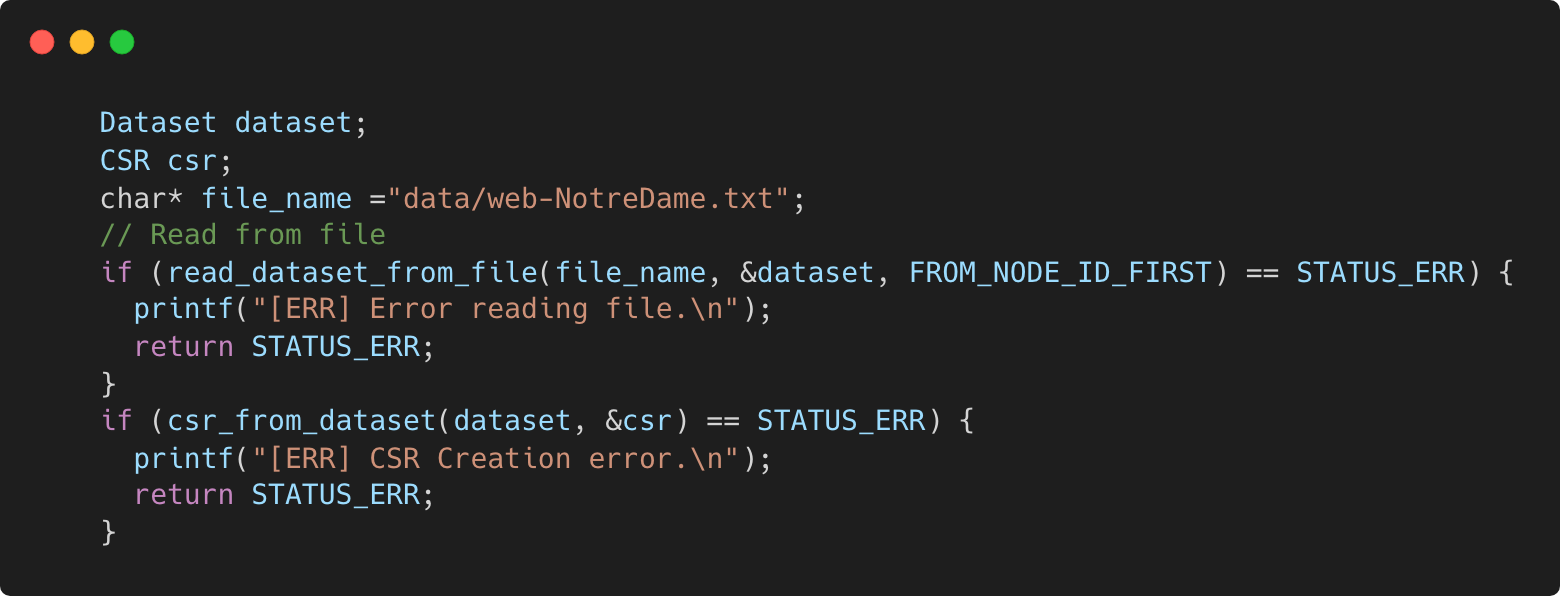
\includegraphics[scale=0.2]{img/main-1-ex.png}
\end{center}
will load the dataset from file data/web-NotreDame.txt into the dataset variable and it will create the CSR struct from the given dataset.

After that, user can use the CSR for compute a rank. For example, if user wants to compute PageRank he can firstly make the CSR stochastic with the appropriate function and then call the page\_rank function.
\begin{center}
    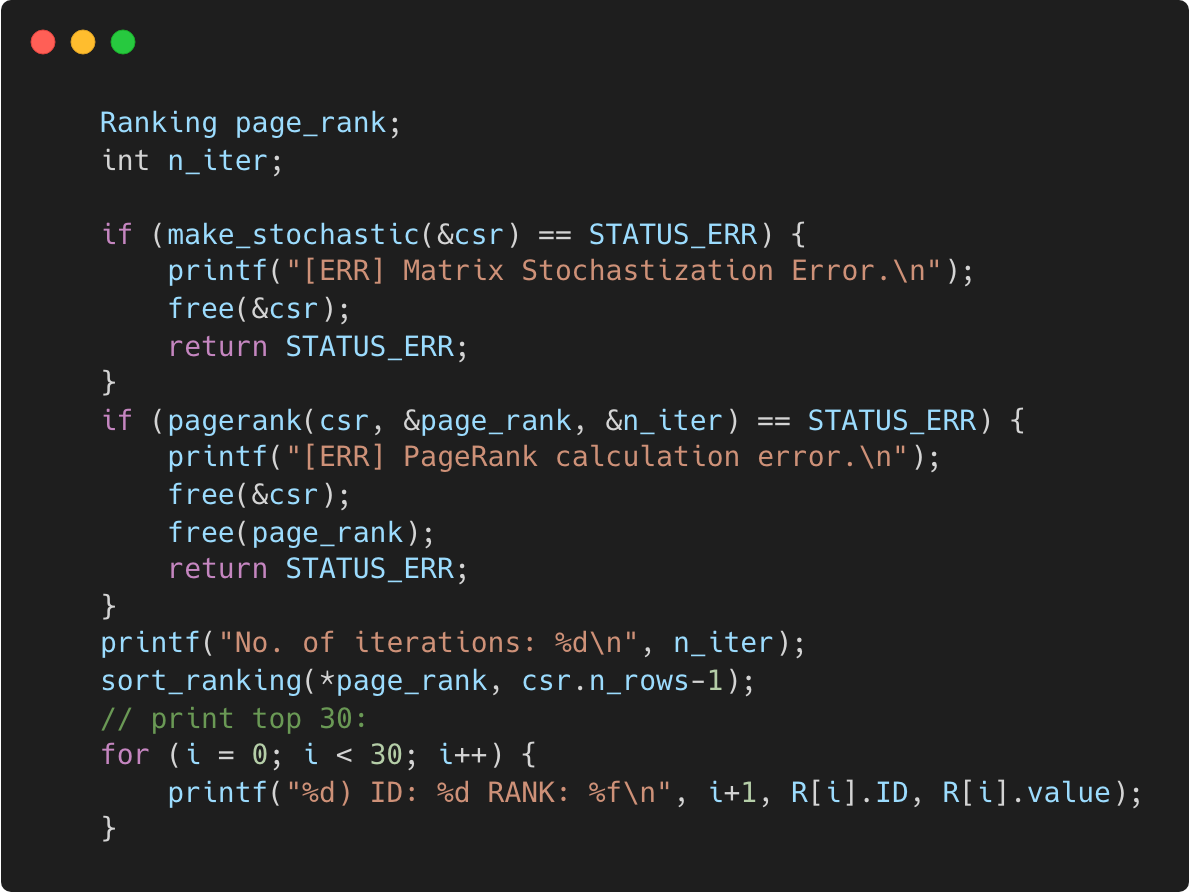
\includegraphics[scale=0.2]{img/main-2-ex.png}
\end{center}
The previous image shows how to use to print out the top k pages: user must sort the ranking and then iterate over the Ranking array.
The Jaccard Similarity between two Ranking can be computed by calling:  
\begin{center}
    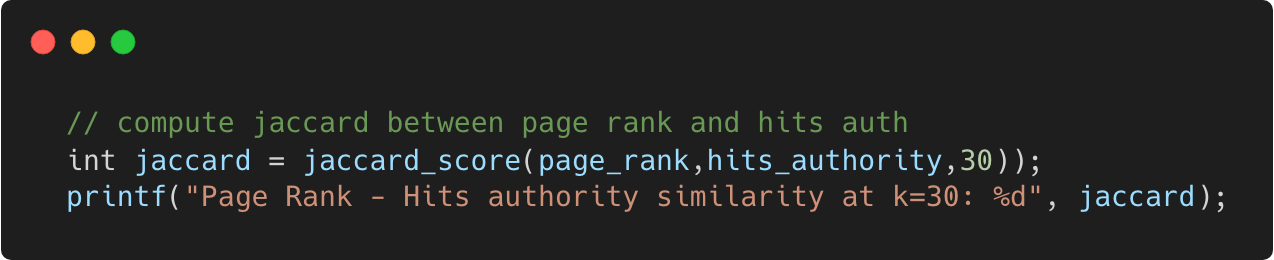
\includegraphics[scale=0.2]{img/main-3-ex.png}
\end{center}

\subsection{The main file}

\subsection{Building the demo}
The demo program can be builded by launching the make command from the command line.
User can open a new terminal window from the project directory and launch the next command:
\begin{verbatim}make\end{verbatim}
for building the project. This command reads the MakeFile and executes the default rule.

For using the mmap feature, user must call from the terminal
\begin{verbatim}make mmap\end{verbatim}
The two commands mentioned before generates, respectively, two executable files:
\begin{enumerate}
    \item {\bf ranking:} the demo program with standard feature.
    \item {\bf ranking-mmap:} the demo program with mmap feature.
\end{enumerate}

\subsection{Executing the demo}
User must launch the program passing two parameters as arguments: the first one is the path of the input file and the second one is an integer K used for print out the K-top ranking and to compute similarity, for example:
\begin{verbatim}./ranking data/web-NotreDame.txt 30\end{verbatim}
it will launch the default version of program (without mmap) using the dataset data/web-NotreDame.txt and with the top 30 ranking printed out.
\section{Some results}
Now we analyze the dataset web-NotreDame. \\
With error threshold at 10e-8 and d=0.85 PageRank converges at iteration 66.\\
With error threshold at 10e-8 Hits converges at iteration 93.\\
The top 30 pages returned by page rank are:
\begin{verbatim}
1) ID: 1963 RANK: 0.002069
2) ID: 0 RANK: 0.002066
3) ID: 10336 RANK: 0.001882
4) ID: 212843 RANK: 0.001438
5) ID: 124802 RANK: 0.001217
6) ID: 12129 RANK: 0.001025
7) ID: 191267 RANK: 0.001009
8) ID: 32830 RANK: 0.001005
9) ID: 83606 RANK: 0.000905
10) ID: 1973 RANK: 0.000872
11) ID: 142732 RANK: 0.000861
12) ID: 24823 RANK: 0.000822
13) ID: 143218 RANK: 0.000792
14) ID: 3451 RANK: 0.000761
15) ID: 31331 RANK: 0.000691
16) ID: 149039 RANK: 0.000663
17) ID: 140170 RANK: 0.000536
18) ID: 12838 RANK: 0.000516
19) ID: 81878 RANK: 0.000512
20) ID: 226950 RANK: 0.000457
21) ID: 73859 RANK: 0.000403
22) ID: 292009 RANK: 0.000399
23) ID: 63364 RANK: 0.000366
24) ID: 24944 RANK: 0.000365
25) ID: 88448 RANK: 0.000354
26) ID: 88118 RANK: 0.000349
27) ID: 10335 RANK: 0.000336
28) ID: 10331 RANK: 0.000323
29) ID: 143082 RANK: 0.000309
30) ID: 32833 RANK: 0.000307
\end{verbatim}
The top 30 pages returned by HITS are:
\begin{verbatim}
HITS AUTHORITY:
1) ID: 12129 RANK: 0.011848
2) ID: 199031 RANK: 0.003976
3) ID: 235904 RANK: 0.003975
4) ID: 151241 RANK: 0.003940
5) ID: 193592 RANK: 0.003939
6) ID: 155590 RANK: 0.003928
7) ID: 198328 RANK: 0.003927
8) ID: 199030 RANK: 0.001340
9) ID: 199029 RANK: 0.001321
10) ID: 199028 RANK: 0.001321
11) ID: 151240 RANK: 0.001315
12) ID: 151238 RANK: 0.001315
13) ID: 151239 RANK: 0.001315
14) ID: 155589 RANK: 0.001313
15) ID: 155587 RANK: 0.001313
16) ID: 155588 RANK: 0.001306
17) ID: 236095 RANK: 0.000551
18) ID: 260644 RANK: 0.000550
19) ID: 260645 RANK: 0.000550
20) ID: 260646 RANK: 0.000550
21) ID: 260647 RANK: 0.000550
22) ID: 260648 RANK: 0.000550
23) ID: 260649 RANK: 0.000550
24) ID: 260650 RANK: 0.000550
25) ID: 260651 RANK: 0.000550
26) ID: 260652 RANK: 0.000550
27) ID: 260653 RANK: 0.000550
28) ID: 260654 RANK: 0.000550
29) ID: 260655 RANK: 0.000550
30) ID: 260656 RANK: 0.000550

HITS HUB:
1) ID: 260552 RANK: 0.000304
2) ID: 236095 RANK: 0.000304
3) ID: 260634 RANK: 0.000304
4) ID: 260635 RANK: 0.000304
5) ID: 260636 RANK: 0.000304
6) ID: 260637 RANK: 0.000304
7) ID: 260638 RANK: 0.000304
8) ID: 260639 RANK: 0.000304
9) ID: 260640 RANK: 0.000304
10) ID: 260641 RANK: 0.000304
11) ID: 260642 RANK: 0.000304
12) ID: 260643 RANK: 0.000304
13) ID: 260644 RANK: 0.000304
14) ID: 260588 RANK: 0.000304
15) ID: 260589 RANK: 0.000304
16) ID: 260590 RANK: 0.000304
17) ID: 260591 RANK: 0.000304
18) ID: 260592 RANK: 0.000304
19) ID: 260593 RANK: 0.000304
20) ID: 260594 RANK: 0.000304
21) ID: 260595 RANK: 0.000304
22) ID: 260596 RANK: 0.000304
23) ID: 260597 RANK: 0.000304
24) ID: 260598 RANK: 0.000304
25) ID: 260599 RANK: 0.000304
26) ID: 260645 RANK: 0.000304
27) ID: 260646 RANK: 0.000304
28) ID: 260647 RANK: 0.000304
29) ID: 260600 RANK: 0.000304
30) ID: 260648 RANK: 0.000304
\end{verbatim}
The top 30 pages returned by InDegree are:
\begin{verbatim}
1) ID: 12129 RANK: 0.032914
2) ID: 0 RANK: 0.023391
3) ID: 124802 RANK: 0.021570
4) ID: 31331 RANK: 0.013201
5) ID: 140170 RANK: 0.013137
6) ID: 199031 RANK: 0.010982
7) ID: 235904 RANK: 0.010978
8) ID: 151241 RANK: 0.010966
9) ID: 193592 RANK: 0.010963
10) ID: 155590 RANK: 0.010939
11) ID: 198328 RANK: 0.010935
12) ID: 191267 RANK: 0.007205
13) ID: 12838 RANK: 0.006656
14) ID: 81878 RANK: 0.006472
15) ID: 1973 RANK: 0.006054
16) ID: 142732 RANK: 0.005805
17) ID: 143218 RANK: 0.005323
18) ID: 46468 RANK: 0.005142
19) ID: 24823 RANK: 0.004390
20) ID: 3451 RANK: 0.003887
21) ID: 212843 RANK: 0.003804
22) ID: 212812 RANK: 0.003801
23) ID: 73875 RANK: 0.003785
24) ID: 307409 RANK: 0.003776
25) ID: 73874 RANK: 0.003776
26) ID: 307408 RANK: 0.003770
27) ID: 73859 RANK: 0.003745
28) ID: 292009 RANK: 0.003739
29) ID: 199030 RANK: 0.003678
30) ID: 199029 RANK: 0.003663
\end{verbatim}

The Jaccard similarity between ranking are:

\begin{tabular}{||c c c c||} 
    \hline
    K & PageRank - HITS & PageRank - InDegree & HITS - InDegree \\ [0.5ex] 
    \hline\hline
    10 & 0.052632 & 0.176471 & 0.428571 \\
    20 & 0.025641 & 0.481481 & 0.212121 \\
    30 & 0.016949 & 0.363636 & 0.176471 \\ [1ex] 
    \hline
\end{tabular}

The next two images will show how the jaccard score change when K change: the first one shows the value of the jaccard score for k from 1 to 100. The second image shows how jaccard score behaves for k from 1 to the number of nodes in the dataset.

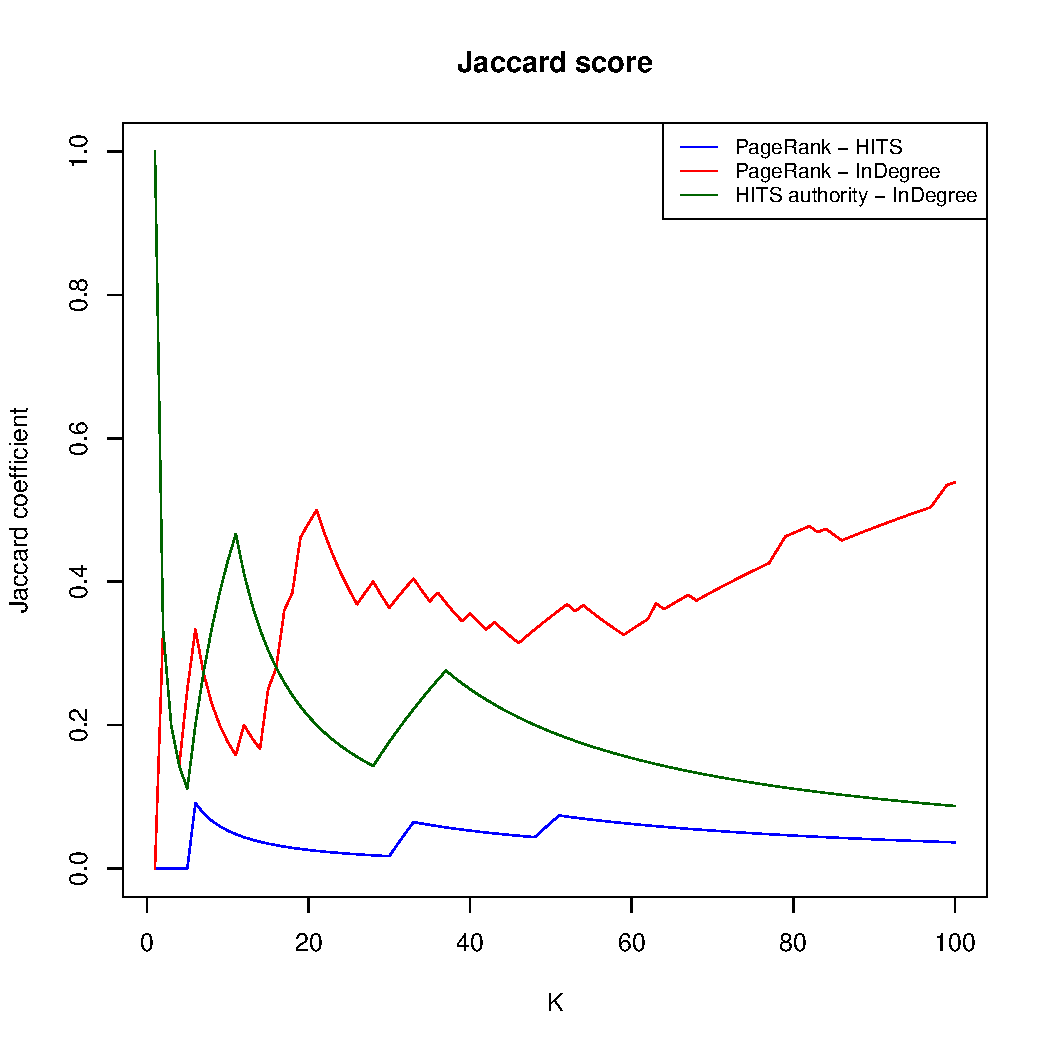
\includegraphics[scale=0.8]{img/jaccard-100.pdf}

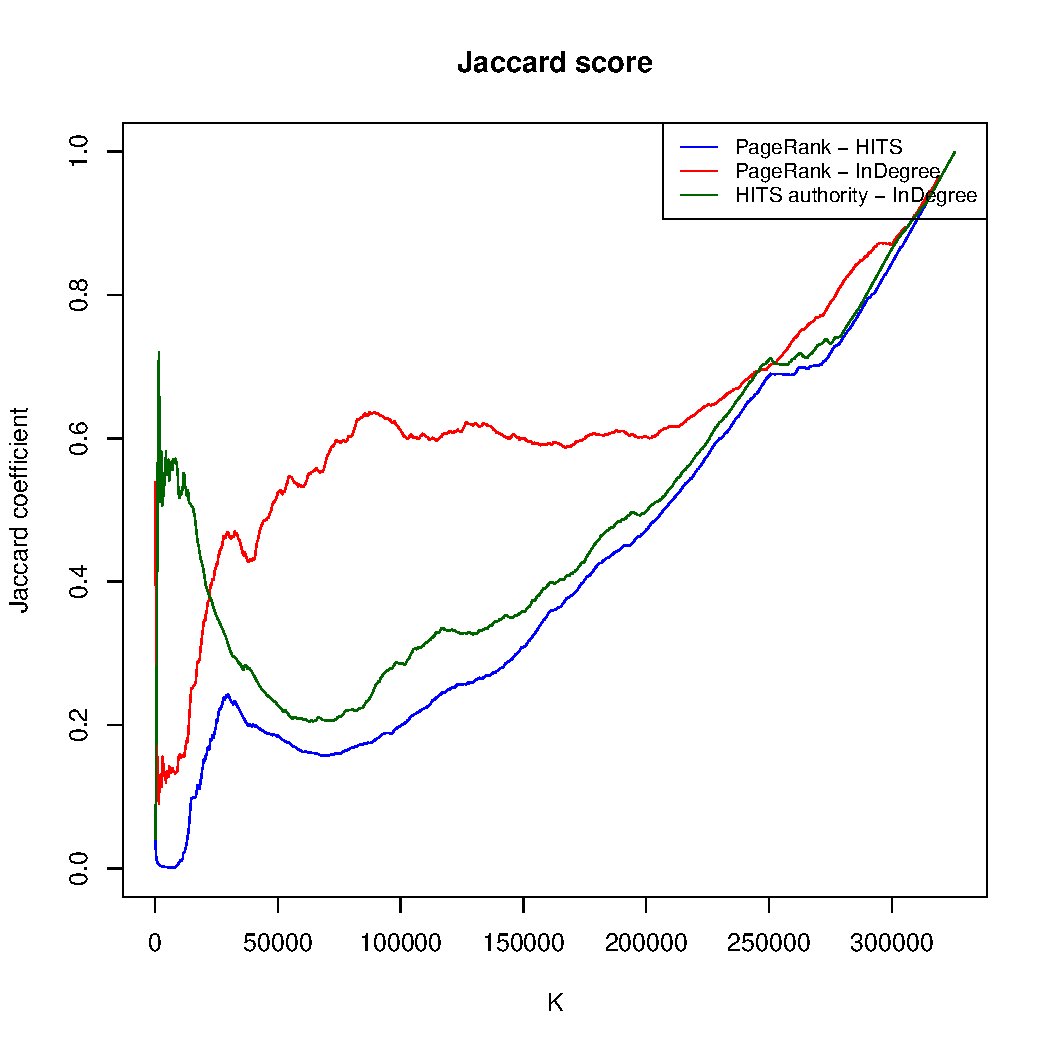
\includegraphics[scale=0.8]{img/jaccard-all.pdf}

\section{Conclusion}
We have seen an efficient implementation of PageRank and HITS in C language, using the mmap capabilities.\\
We have computed the jaccard similarity between the ranking, and we seen that HITS and InDegree are more similiar for lower k. When K becomes bigger, this similarity decreases and the similarity between PageRank and InDegree increase.\\
HITS and PageRank, instead, are not very similiar.\\
Talking about performance, from the output of the program we can see that the PageRank computation is faster than HITS (). This because HITS output 2 different ranking and the computation is a bit more complex.\\
Here the logging of the program:\\
\begin{verbatim}
    [INFO] Done reading dataset. Time: 0.371658
    [INFO] Reading transposed dataset...
    [INFO] Done reading transpose dataset. Time: 0.554761
    [INFO] Reading dataset...
    [INFO] Generating CSR...
    [INFO] Done generating CSR. Time: 0.014086
    [INFO] Generating transposed CSR...
    [INFO] Done generating transpose CSR. Time: 0.024232
    [INFO] Generating transposed CSR...
    [INFO] Done generating transpose CSR. Time: 0.016360
    [INFO] Stochastization...
    [INFO] Done stochastization. Time: 0.006181
    [INFO] Computing Pagerank...
    [INFO] PAGERANK: Computing... 
    [INFO] PAGERANK: Done computing. Time: 0.208020
    [INFO] PAGERANK: No. of iterations: 66
    [INFO] PAGERANK: sorting rank entries...
    [INFO] PAGERANK: done sorting rank entries. Time: 0.025548
    [INFO] Done computing Pagerank. Total time spent: 0.233604
    [INFO] Computing HITS...
    [INFO] HITS: Computing... 
    [INFO] HITS: Done computing. Time: 0.800050
    [INFO] HITS: No. of iterations: 93
    [INFO] HITS: sorting rank entries...
    [INFO] HITS: done sorting rank entries. Time: 0.035991
    [INFO] Done computing HITS. Total time spent: 0.836071
    [INFO] Computing INDEGREE...
    [INFO] INDEGREE: Computing...
    [INFO] INDEGREE: Done computing. Time: 0.001482
    [INFO] INDEGREE: sorting rank entries...
    [INFO] INDEGREE: done sorting rank entries. Time: 0.005886
    [INFO] Done computing INDEGREE. Total time spent: 0.007383
\end{verbatim}

We notice also that PageRank converges faster than HITS. This because HITS needs that both the errors of hubs and authority are under the threshold.
\section{Future works and improvement}

A nice to have feature could be the possibility to parameterize some variables, such as:
\begin{itemize}
    \item dumping factor
    \item error threshold
    \item error function
\end{itemize}
This permits more freedom from user perspective.
\newpage

% -----------------------------
\bibliographystyle{abbrv} 
\bibliography{references.bib} % Bibliography

\end{document}